\documentclass[12pt, a4paper]{article}

% 中文支持
\usepackage{ctex}

% 页面设置
\usepackage{geometry}
\geometry{left=2.5cm, right=2.5cm, top=2.5cm, bottom=2.5cm}

% 数学支持
\usepackage{amsmath, amssymb, amsthm}

% 绘图
\usepackage{tikz}
\usetikzlibrary{arrows.meta, positioning, shapes.geometric, calc, decorations.pathreplacing}

% 代码高亮
\usepackage{listings}
\lstset{
    basicstyle=\ttfamily\small,
    keywordstyle=\color{blue},
    commentstyle=\color{gray},
    numbers=left,
    numberstyle=\tiny,
    frame=single,
    breaklines=true
}

% 表格
\usepackage{booktabs}

% 超链接
\usepackage{hyperref}
\hypersetup{
    colorlinks=true,
    linkcolor=blue,
    urlcolor=blue
}

% 图片
\usepackage{graphicx}
\graphicspath{{figures/}}

% 定理环境
\newtheorem{definition}{定义}[section]
\newtheorem{theorem}{定理}[section]
\newtheorem{lemma}{引理}[section]
\newtheorem{example}{例}[section]

% 标题信息
\title{算法图论复习笔记}
\author{Yibo Liu}
\date{\today}

\begin{document}

\maketitle

\tableofcontents
\newpage

%========================================
% 第一章：图论基础
%========================================

\section{图论基础}

\subsection{图的基本概念}

\begin{definition}[图、顶点、边]
一个\textbf{图} $G$ 由两个有限集合组成：
\begin{itemize}
    \item 一个对象集合 $V = \{v_1, v_2, v_3, \dots, v_m\}$，称为\textbf{顶点}（vertices），也称为\textbf{点}（points）或\textbf{节点}（nodes）
    \item 另一个集合 $E = \{e_1, e_2, e_3, \dots, e_n\}$，其中的元素称为\textbf{边}（edges），也称为\textbf{线}（lines）或\textbf{弧}（arcs）
\end{itemize}

集合 $V(G)$ 称为图 $G$ 的\textbf{顶点集合}（vertex set），集合 $E(G)$ 称为图 $G$ 的\textbf{边集合}（edge set）。

并且 $V \cap E = \varnothing$，即\textbf{顶点集合和边集合互不相交}。

通常，一个图表示为 $G = (V(G), E(G))$，或者更简单写作 $G = (V, E)$。
\end{definition}

\begin{definition}[端点、关联、邻接、环、多重边]
每一条边 $e \in E$ 都对应于顶点集合 $V$ 中的\textbf{两个顶点}，这两个顶点称为该边的\textbf{端点}（endpoints）。

\begin{itemize}
    \item \textbf{关联（incident）}：一条边关联于它的两个端点，或者说这条边在两个端点之间
    \item \textbf{邻接（adjacent）}：如果两个顶点 $u$ 和 $v$ 之间存在一条边，则称 $u$ 和 $v$ 邻接，或称为邻居（neighbors）
    \item \textbf{环（loop）}：如果一条边的两个端点是同一个顶点
    \item \textbf{多重边（multiple edge）}：如果存在另一条具有相同端点的边
\end{itemize}
\end{definition}

\subsection{顶点和边的表示}

\textbf{顶点的表示：} 给定一个图 $G$，我们通常用整数来表示顶点。如果图 $G$ 有 $n$ 个顶点，则 $V(G) = [n]$。

\textbf{边的表示：} 设 $G$ 是一个图，$\{u, v\}$ 是一条边。因为 $\{u, v\}$ 是一个两个元素的集合，所以 $\{u, v\} = \{v, u\}$，因此通常更方便写作 $uv$ 或 $vu$。

如果 $e = uv$ 是图 $G$ 的一条边，则称：
\begin{itemize}
    \item $u$ 和 $v$ 在 $G$ 中\textbf{邻接}
    \item 边 $e$ \textbf{连接}（joins）顶点 $u$ 和 $v$
\end{itemize}

\subsection{图的示例}

\begin{example}
一个图 $G$ 由以下集合定义：

顶点集合：$V(G) = \{u, v, w, x, y, z\}$

边集合：$E(G) = \{uv, uw, wx, xy, xz\}$

\begin{center}
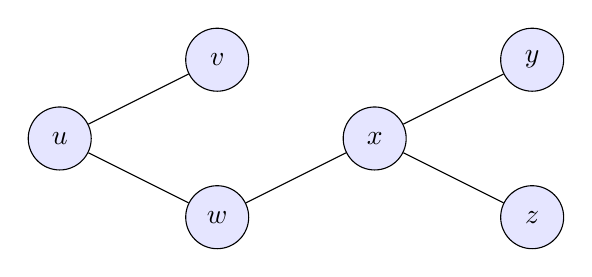
\begin{tikzpicture}[
    vertex/.style={circle, draw, minimum size=0.8cm, fill=blue!10}
]
    \node[vertex] (u) at (0, 1) {$u$};
    \node[vertex] (v) at (2, 2) {$v$};
    \node[vertex] (w) at (2, 0) {$w$};
    \node[vertex] (x) at (4, 1) {$x$};
    \node[vertex] (y) at (6, 2) {$y$};
    \node[vertex] (z) at (6, 0) {$z$};

    \draw (u) -- (v);
    \draw (u) -- (w);
    \draw (w) -- (x);
    \draw (x) -- (y);
    \draw (x) -- (z);
\end{tikzpicture}
\end{center}
\end{example}

\begin{example}[判断是否为图]
\textbf{(1)} 设 $V = \{1, 2, 3, 4\}$，$E = \{\{1,2\}, \{1,3\}, \{3,2\}, \{4,4\}\}$，则 $G(V, E)$ 是一个图。

\begin{center}
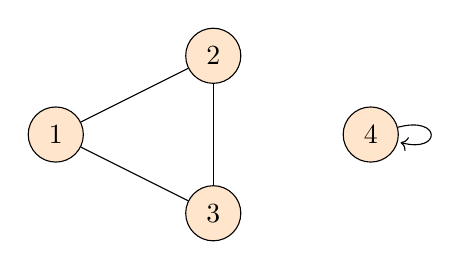
\begin{tikzpicture}[
    vertex/.style={circle, draw, minimum size=0.7cm, fill=orange!20}
]
    \node[vertex] (1) at (0, 0) {1};
    \node[vertex] (2) at (2, 1) {2};
    \node[vertex] (3) at (2, -1) {3};
    \node[vertex] (4) at (4, 0) {4};

    \draw (1) -- (2);
    \draw (1) -- (3);
    \draw (2) -- (3);
    \draw (4) edge[loop right] (4);  % 环
\end{tikzpicture}
\end{center}

\textbf{说明：} 边 $\{4,4\}$ 是一个\textbf{环}（loop），顶点 4 与自身相连。

\vspace{0.5cm}

\textbf{(2)} 设 $V = \{1, 2, 3, 4\}$，$E = \{\{1,5\}, \{2,3\}\}$，则 $G(V, E)$ \textbf{不是一个图}。

\textbf{原因：} 5 不在顶点集合 $V$ 中，所以 $\{1, 5\}$ 不是合法的边。

\vspace{0.5cm}

\textbf{(3)} 一个具有 5 个顶点和 8 条边的图称为 \textbf{$(5, 8)$ 图}。

\begin{center}
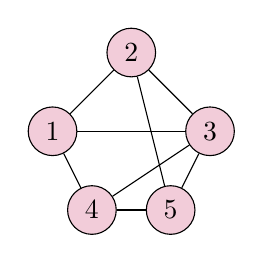
\begin{tikzpicture}[
    vertex/.style={circle, draw, minimum size=0.6cm, fill=purple!20}
]
    \node[vertex] (1) at (0, 1) {1};
    \node[vertex] (2) at (1, 2) {2};
    \node[vertex] (3) at (2, 1) {3};
    \node[vertex] (4) at (0.5, 0) {4};
    \node[vertex] (5) at (1.5, 0) {5};

    \draw (1) -- (2);
    \draw (1) -- (3);
    \draw (1) -- (4);
    \draw (2) -- (3);
    \draw (2) -- (5);
    \draw (3) -- (4);
    \draw (3) -- (5);
    \draw (4) -- (5);
\end{tikzpicture}
\end{center}
\end{example}

\subsection{简单图}

我们主要关注所谓的\textbf{简单图}（simple graphs），即\textbf{没有自环（loop）也没有多重边（multiple edges）}的图。

\begin{definition}[简单图]
一个图 $G$ 称为\textbf{简单图}（simple），如果：
\begin{enumerate}
    \item 每一条边在 $E(G)$ 中都有\textbf{两个不同的端点}（即没有环）
    \item 对于任意两个顶点 $u, v \in V(G)$，\textbf{最多只有一条边}同时连接 $u$ 和 $v$（即没有多重边）
\end{enumerate}
\end{definition}

在讨论简单图时，通常用\textbf{边的两个端点来标记该边}。因此我们会说：
\begin{itemize}
    \item \textbf{边 $\{u, v\}$} 或 \textbf{边 $uv$} 来表示端点为 $u$ 和 $v$ 的边
    \item 注意：$uv = vu$，它们表示\textbf{同一条边}
\end{itemize}

根据简单图的两个性质：
\begin{itemize}
    \item 每条边由\textbf{两个顶点标记}
    \item 每个标记\textbf{最多对应一条边}
\end{itemize}

因此不会产生混淆。换句话说，在顶点集合为 $V$ 的简单图中，所有可能的边集合与 $\binom{|V|}{2}$ 个\textbf{顶点的无序对}（unordered pairs）之间存在\textbf{一一对应关系}（bijection）。

\begin{theorem}[简单图的最大边数]
一个具有 $n$ 个顶点的简单图，最多有
\[
\binom{n}{2} = \frac{n(n-1)}{2}
\]
条边。
\end{theorem}

\begin{theorem}[推论 1.6：简单图的数量]
对于任意有限顶点集合 $V$，具有顶点集合 $V$ 的不同\textbf{简单图}共有：
\[
2^{\binom{|V|}{2}}
\]
个。
\end{theorem}

\textbf{证明：} 根据定理 1.5，对于顶点集合为 $V$ 的简单图，最多可以有 $\binom{|V|}{2}$ 条边。对于每一条可能的边，有两种选择：
\begin{itemize}
    \item \textbf{包含该边}
    \item \textbf{不包含该边}
\end{itemize}
因此，不同简单图的总数为 $2^{\binom{|V|}{2}}$ 个。

%----------------------------------------
% 特殊图
%----------------------------------------

\subsection{特殊图}

一些图会反复出现，因此被赋予了名称。

\begin{example}[空图 $E_n$]
一个只包含\textbf{孤立顶点}（isolated vertices）的图称为\textbf{空图}（null graph）。空图中的边集合为空。

具有 $n$ 个顶点的空图记为 $E_n$，且：
\[
V(E_n) = [n], \quad E(E_n) = \varnothing
\]

\begin{center}
\begin{tikzpicture}[
    vertex/.style={circle, draw, minimum size=0.5cm, fill=gray!30}
]
    % E_5
    \node[vertex] (1) at (0, 0) {1};
    \node[vertex] (2) at (0.8, 0) {2};
    \node[vertex] (3) at (1.6, 0) {3};
    \node[vertex] (4) at (2.4, 0) {4};
    \node[vertex] (5) at (3.2, 0) {5};
    \node[below=0.8cm of 3] {$E_5$：空图（5个孤立顶点）};
\end{tikzpicture}
\end{center}
\end{example}

\begin{example}[完全图 $K_n$]
如果一个简单图 $G$ 满足\textbf{每一个顶点都与其他所有顶点相连}，则称为\textbf{完全图}（complete graph）。

也就是说，任意两个不同顶点之间\textbf{恰好有一条边}。

完全图记作 $K_n$，且：
\[
V(K_n) = [n], \quad E(K_n) = \{uv : u, v \in [n], u \neq v\}
\]

\begin{center}
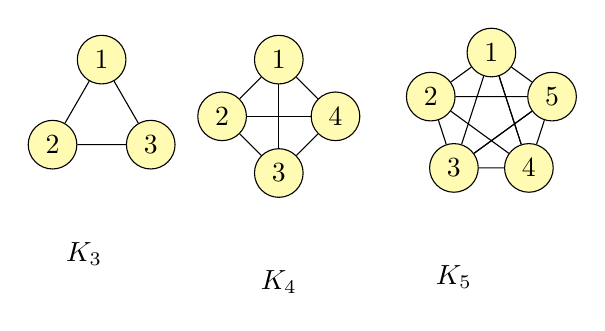
\begin{tikzpicture}[
    vertex/.style={circle, draw, minimum size=0.5cm, fill=yellow!30},
    scale=0.9
]
    % K_3
    \begin{scope}[shift={(0,0)}]
        \node[vertex] (1) at (90:0.8) {1};
        \node[vertex] (2) at (210:0.8) {2};
        \node[vertex] (3) at (330:0.8) {3};
        \draw (1) -- (2) -- (3) -- (1);
        \node[below=0.8cm of 2, xshift=0.4cm] {$K_3$};
    \end{scope}

    % K_4
    \begin{scope}[shift={(2.5,0)}]
        \node[vertex] (1) at (90:0.8) {1};
        \node[vertex] (2) at (180:0.8) {2};
        \node[vertex] (3) at (270:0.8) {3};
        \node[vertex] (4) at (0:0.8) {4};
        \draw (1) -- (2) -- (3) -- (4) -- (1);
        \draw (1) -- (3);
        \draw (2) -- (4);
        \node[below=0.8cm of 3] {$K_4$};
    \end{scope}

    % K_5
    \begin{scope}[shift={(5.5,0)}]
        \node[vertex] (1) at (90:0.9) {1};
        \node[vertex] (2) at (162:0.9) {2};
        \node[vertex] (3) at (234:0.9) {3};
        \node[vertex] (4) at (306:0.9) {4};
        \node[vertex] (5) at (18:0.9) {5};
        \draw (1) -- (2) -- (3) -- (4) -- (5) -- (1);
        \draw (1) -- (3) -- (5) -- (2) -- (4) -- (1);
        \draw (1) -- (4);
        \draw (2) -- (5);
        \draw (3) -- (5);
        \node[below=0.8cm of 3] {$K_5$};
    \end{scope}
\end{tikzpicture}
\end{center}

\textbf{注意：} $K_n$ 有 $\binom{n}{2} = \frac{n(n-1)}{2}$ 条边。
\end{example}

\begin{example}[路径图 $P_n$ 和环图 $C_n$]
\textbf{路径图} $P_n$ 表示具有 $n$ 个顶点的路径：
\[
V(P_n) = [n], \quad E(P_n) = \{uv : u, v \in [n], |u-v| = 1\}
\]

\textbf{环图} $C_n$ 表示具有 $n \geq 3$ 个顶点的环：
\[
V(C_n) = [n], \quad E(C_n) = \{uv : u, v \in [n], |u-v| = 1\} \cup \{1n\}
\]

\begin{center}
\begin{tikzpicture}[
    vertex/.style={circle, draw, minimum size=0.5cm, fill=cyan!30}
]
    % P_4 路径图
    \begin{scope}[shift={(0,0)}]
        \node[vertex] (1) at (0, 0) {1};
        \node[vertex] (2) at (1, 0) {2};
        \node[vertex] (3) at (2, 0) {3};
        \node[vertex] (4) at (3, 0) {4};
        \draw (1) -- (2) -- (3) -- (4);
        \node[below=0.5cm of 2, xshift=0.5cm] {$P_4$：路径图};
    \end{scope}

    % C_3 环图
    \begin{scope}[shift={(5,0)}]
        \node[vertex] (1) at (90:0.7) {1};
        \node[vertex] (2) at (210:0.7) {2};
        \node[vertex] (3) at (330:0.7) {3};
        \draw (1) -- (2) -- (3) -- (1);
        \node[below=0.6cm of 2, xshift=0.35cm] {$C_3$};
    \end{scope}

    % C_4 环图
    \begin{scope}[shift={(7.5,0)}]
        \node[vertex] (1) at (0, 0.7) {1};
        \node[vertex] (2) at (0.7, 0) {2};
        \node[vertex] (3) at (0, -0.7) {3};
        \node[vertex] (4) at (-0.7, 0) {4};
        \draw (1) -- (2) -- (3) -- (4) -- (1);
        \node[below=0.6cm of 3] {$C_4$};
    \end{scope}

    % C_5 环图
    \begin{scope}[shift={(10.5,0)}]
        \node[vertex] (1) at (90:0.7) {1};
        \node[vertex] (2) at (162:0.7) {2};
        \node[vertex] (3) at (234:0.7) {3};
        \node[vertex] (4) at (306:0.7) {4};
        \node[vertex] (5) at (18:0.7) {5};
        \draw (1) -- (2) -- (3) -- (4) -- (5) -- (1);
        \node[below=0.6cm of 3] {$C_5$};
    \end{scope}
\end{tikzpicture}
\end{center}

\textbf{注意：}
\begin{itemize}
    \item $P_n$ 有 $n-1$ 条边
    \item $C_n$ 有 $n$ 条边
\end{itemize}
\end{example}

\begin{example}[简单图 vs 非简单图]
\begin{center}
\begin{tikzpicture}[
    vertex/.style={circle, draw, minimum size=0.7cm},
    simple/.style={vertex, fill=green!20},
    nonsimple/.style={vertex, fill=red!20}
]
    % 简单图
    \node[simple] (a1) at (0, 0) {$a$};
    \node[simple] (b1) at (1.5, 0) {$b$};
    \node[simple] (c1) at (0.75, 1.2) {$c$};
    \draw (a1) -- (b1) -- (c1) -- (a1);
    \node[below=0.5cm of a1, anchor=north west] {简单图};

    % 非简单图（有环）
    \node[nonsimple] (a2) at (4, 0) {$a$};
    \node[nonsimple] (b2) at (5.5, 0) {$b$};
    \node[nonsimple] (c2) at (4.75, 1.2) {$c$};
    \draw (a2) -- (b2) -- (c2) -- (a2);
    \draw (a2) edge[loop left] (a2);
    \node[below=0.5cm of a2, anchor=north west] {有环（非简单图）};

    % 非简单图（有多重边）
    \node[nonsimple] (a3) at (8, 0) {$a$};
    \node[nonsimple] (b3) at (9.5, 0) {$b$};
    \node[nonsimple] (c3) at (8.75, 1.2) {$c$};
    \draw (a3) -- (b3) -- (c3) -- (a3);
    \draw (a3) to[bend left=30] (b3);
    \node[below=0.5cm of a3, anchor=north west] {有多重边（非简单图）};
\end{tikzpicture}
\end{center}
\end{example}

\subsection{$(p, q)$ 图与平凡图}

\begin{definition}[$(p, q)$ 图]
一个具有 $p$ 个顶点、$q$ 条边的图称为\textbf{$(p, q)$ 图}。
\end{definition}

\begin{definition}[平凡图]
$(1, 0)$ 图称为\textbf{平凡图}（trivial graph），即只有一个顶点、没有边的图。
\end{definition}

\begin{center}
\begin{tikzpicture}[
    vertex/.style={circle, draw, minimum size=0.8cm, fill=gray!20}
]
    \node[vertex] (v) at (0, 0) {$v$};
    \node[below=0.3cm of v] {平凡图：$(1,0)$ 图};
\end{tikzpicture}
\end{center}

\subsection{邻接关系示例}

\begin{center}
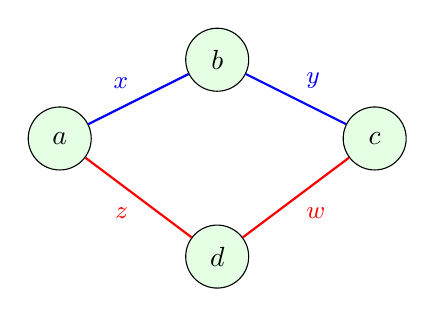
\begin{tikzpicture}[
    vertex/.style={circle, draw, minimum size=0.8cm, fill=green!10},
    edge label/.style={midway, font=\small}
]
    % 顶点
    \node[vertex] (a) at (0, 0) {$a$};
    \node[vertex] (b) at (2, 1) {$b$};
    \node[vertex] (c) at (4, 0) {$c$};
    \node[vertex] (d) at (2, -1.5) {$d$};

    % 边（带标签）
    \draw[thick, blue] (a) -- node[edge label, above left] {$x$} (b);
    \draw[thick, blue] (b) -- node[edge label, above right] {$y$} (c);
    \draw[thick, red] (a) -- node[edge label, below left] {$z$} (d);
    \draw[thick, red] (c) -- node[edge label, below right] {$w$} (d);
\end{tikzpicture}
\end{center}

\textbf{说明：}
\begin{itemize}
    \item 顶点 $a$ 和 $b$ 是\textbf{邻接的}，$a$ 和 $c$ \textbf{不是邻接的}
    \item 边 $x$ 和 $y$ 是\textbf{邻接的}（共享顶点 $b$），但 $x$ 和 $z$ \textbf{不是邻接的}
    \item 虽然在图示中边 $x$ 和边 $w$ 可能相交，但这个交点\textbf{不是图的顶点}
\end{itemize}

%----------------------------------------
% 重要概念补充
%----------------------------------------

\subsection{重要概念}

\begin{definition}[度数（Degree）]
顶点 $v$ 的\textbf{度数} $\deg(v)$ 是与 $v$ 关联的边的数目。

\textbf{注意：} 环对度数的贡献为 2。
\end{definition}

\begin{theorem}[握手定理]
设 $G = (V, E)$ 是一个图，则：
\[
\sum_{v \in V} \deg(v) = 2|E|
\]
即所有顶点的度数之和等于边数的两倍。
\end{theorem}

\begin{definition}[路径（Path）、通道（Walk）、环（Cycle）]
\begin{itemize}
    \item \textbf{通道（walk）}：顶点和边交替的序列 $v_0, e_1, v_1, e_2, \dots, e_k, v_k$，其中每条边关联其前后的两个顶点
    \item \textbf{路径（path）}：所有顶点都不重复的通道
    \item \textbf{环/圈（cycle）}：起点和终点相同，且其他顶点都不重复的通道
\end{itemize}
\end{definition}

\begin{definition}[连通图（Connected Graph）]
如果图中任意两个顶点之间都存在路径，则称该图为\textbf{连通图}。
\end{definition}

\begin{definition}[二部图（Bipartite Graph）]
如果图 $G$ 的顶点集 $V$ 可以划分为两个不相交的子集 $A$ 和 $B$，使得每条边都连接 $A$ 中的一个顶点和 $B$ 中的一个顶点，则称 $G$ 为\textbf{二部图}。
\end{definition}

\begin{center}
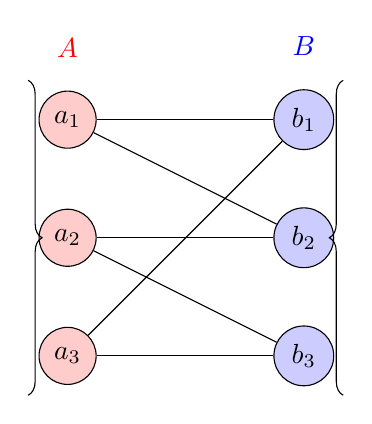
\begin{tikzpicture}[
    vertex/.style={circle, draw, minimum size=0.7cm},
    setA/.style={vertex, fill=red!20},
    setB/.style={vertex, fill=blue!20}
]
    % 二部图示例
    \node[setA] (a1) at (0, 1.5) {$a_1$};
    \node[setA] (a2) at (0, 0) {$a_2$};
    \node[setA] (a3) at (0, -1.5) {$a_3$};

    \node[setB] (b1) at (3, 1.5) {$b_1$};
    \node[setB] (b2) at (3, 0) {$b_2$};
    \node[setB] (b3) at (3, -1.5) {$b_3$};

    \draw (a1) -- (b1);
    \draw (a1) -- (b2);
    \draw (a2) -- (b2);
    \draw (a2) -- (b3);
    \draw (a3) -- (b1);
    \draw (a3) -- (b3);

    % 标注
    \node[above=0.3cm of a1, red] {$A$};
    \node[above=0.3cm of b1, blue] {$B$};

    \draw[decorate, decoration={brace, amplitude=5pt, mirror}] (-0.5, -2) -- (-0.5, 2);
    \draw[decorate, decoration={brace, amplitude=5pt}] (3.5, -2) -- (3.5, 2);
\end{tikzpicture}
\end{center}

%----------------------------------------
% 图的表示方法
%----------------------------------------

\newpage
\subsection{图的表示方法}

\subsubsection{邻接矩阵}

设图 $G$ 有 $n$ 个顶点，邻接矩阵 $A$ 是一个 $n \times n$ 的矩阵：
\[
A[i][j] = \begin{cases}
1 & \text{如果 } (v_i, v_j) \in E \\
0 & \text{否则}
\end{cases}
\]

\textbf{示例：}

\begin{center}
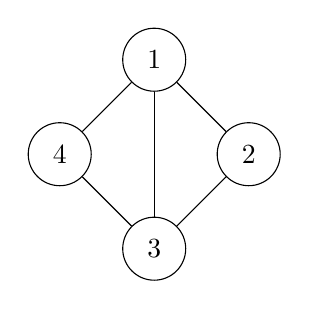
\begin{tikzpicture}[scale=0.8]
    \node[circle, draw, minimum size=0.8cm] (1) at (0, 1.5) {1};
    \node[circle, draw, minimum size=0.8cm] (2) at (1.5, 0) {2};
    \node[circle, draw, minimum size=0.8cm] (3) at (0, -1.5) {3};
    \node[circle, draw, minimum size=0.8cm] (4) at (-1.5, 0) {4};
    \draw (1) -- (2);
    \draw (1) -- (4);
    \draw (2) -- (3);
    \draw (3) -- (4);
    \draw (1) -- (3);
\end{tikzpicture}
\end{center}

对应的邻接矩阵：
\[
A = \begin{pmatrix}
0 & 1 & 1 & 1 \\
1 & 0 & 1 & 0 \\
1 & 1 & 0 & 1 \\
1 & 0 & 1 & 0
\end{pmatrix}
\]

\subsubsection{邻接表}

邻接表为每个顶点存储一个链表，包含所有与之相邻的顶点。

\textbf{空间复杂度：} $O(|V| + |E|)$

\subsubsection{关联矩阵}

对于更大、更复杂的图，或者当我们希望用计算机处理图时，\textbf{关联矩阵}（incidence matrix）是一种有用的表示方式。

设图 $G$ 有 $n$ 个顶点和 $m$ 条边，关联矩阵 $I$ 是一个 $n \times m$ 的矩阵：
\[
I[v][e] = \begin{cases}
1 & \text{如果顶点 } v \text{ 与边 } e \text{ 关联} \\
0 & \text{否则}
\end{cases}
\]

\textbf{示例：}

\begin{center}
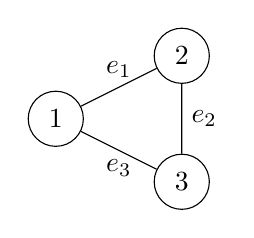
\begin{tikzpicture}[scale=0.8]
    \node[circle, draw, minimum size=0.7cm] (1) at (0, 0) {1};
    \node[circle, draw, minimum size=0.7cm] (2) at (2, 1) {2};
    \node[circle, draw, minimum size=0.7cm] (3) at (2, -1) {3};

    \draw (1) -- node[midway, above] {$e_1$} (2);
    \draw (2) -- node[midway, right] {$e_2$} (3);
    \draw (1) -- node[midway, below] {$e_3$} (3);
\end{tikzpicture}
\end{center}

对应的关联矩阵（行=顶点，列=边）：
\[
I = \begin{array}{c|ccc}
 & e_1 & e_2 & e_3 \\
\hline
1 & 1 & 0 & 1 \\
2 & 1 & 1 & 0 \\
3 & 0 & 1 & 1
\end{array}
\]

\textbf{性质：}
\begin{itemize}
    \item 关联矩阵的每一列恰好有两个 1（每条边关联两个顶点）
    \item 每一行的 1 的个数等于该顶点的度数
\end{itemize}

\subsubsection{图的绘制}

一种方便描述和讨论图的方法是\textbf{在平面上画出图}。对于图 $G$，我们：
\begin{itemize}
    \item 为每个顶点 $v \in V(G)$ 画一个点
    \item 如果 $uv \in E(G)$，则在对应的两个点之间画一条线或曲线
\end{itemize}

\begin{center}
\begin{tikzpicture}[
    vertex/.style={circle, draw, minimum size=0.6cm, fill=blue!15}
]
    % 同一个图的两种画法
    \begin{scope}[shift={(0,0)}]
        \node[vertex] (a) at (0, 0) {$a$};
        \node[vertex] (b) at (1.5, 0) {$b$};
        \node[vertex] (c) at (1.5, 1.2) {$c$};
        \node[vertex] (d) at (0, 1.2) {$d$};
        \draw (a) -- (b) -- (c) -- (d) -- (a);
        \draw (a) -- (c);
        \draw (b) -- (d);
        \node[below=0.4cm of a, xshift=0.75cm] {画法 1};
    \end{scope}

    \begin{scope}[shift={(4,0)}]
        \node[vertex] (a) at (0, 0.6) {$a$};
        \node[vertex] (b) at (1, 1.2) {$b$};
        \node[vertex] (c) at (2, 0.6) {$c$};
        \node[vertex] (d) at (1, 0) {$d$};
        \draw (a) -- (b) -- (c) -- (d) -- (a);
        \draw (a) -- (c);
        \draw (b) -- (d);
        \node[below=0.4cm of d] {画法 2};
    \end{scope}
\end{tikzpicture}
\end{center}

\textbf{注意：} 判断两个图是否相同，关键在于\textbf{顶点与边之间的关联关系}（incidence），而不是顶点或边的具体位置。

%----------------------------------------
% 关联矩阵（完整定义）
%----------------------------------------

\subsubsection{关联矩阵（完整定义）}

\begin{definition}[关联矩阵]
图 $G$ 的\textbf{关联矩阵}（incidence matrix）是一个矩阵：
\begin{itemize}
    \item 行数 $= |V(G)|$（顶点数量）
    \item 列数 $= |E(G)|$（边数量）
\end{itemize}

矩阵元素定义如下：若矩阵元素位于行 $v \in V(G)$、列 $e \in E(G)$，则：
\[
I[v][e] = \begin{cases}
2 & \text{若 } e \text{ 是从 } v \text{ 到自身的自环（loop）} \\
1 & \text{若 } v \text{ 是边 } e \text{ 的两个不同端点之一} \\
0 & \text{其他情况}
\end{cases}
\]
\end{definition}

\begin{example}[图 1.1 的关联矩阵]
图 $G$ 有 $V(G) = \{v_1, v_2, v_3, v_4\}$ 和 7 条边：
\begin{align*}
e_1 &= v_1v_4, \quad e_2 = v_1v_4 \text{（多重边）} \\
e_3 &= v_2v_4, \quad e_4 = v_2v_3 \\
e_5 &= v_1v_2, \quad e_6 = v_3v_4 \\
e_7 &= v_2v_2 \text{（环）}
\end{align*}

\begin{center}
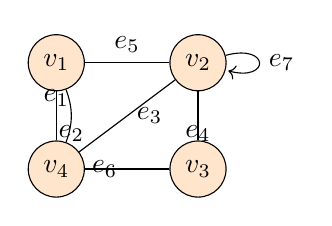
\begin{tikzpicture}[
    vertex/.style={circle, draw, minimum size=0.7cm, fill=orange!20},
    scale=0.9
]
    % 画法 1
    \begin{scope}[shift={(0,0)}]
        \node[vertex] (v1) at (0, 0) {$v_1$};
        \node[vertex] (v2) at (2, 0) {$v_2$};
        \node[vertex] (v3) at (2, -1.5) {$v_3$};
        \node[vertex] (v4) at (0, -1.5) {$v_4$};

        \draw (v1) -- node[midway, above] {$e_1$} (v4);
        \draw (v1) to[bend left=20] node[midway, below] {$e_2$} (v4);
        \draw (v2) -- node[midway, right] {$e_3$} (v4);
        \draw (v2) -- node[midway, below] {$e_4$} (v3);
        \draw (v1) -- node[midway, above] {$e_5$} (v2);
        \draw (v3) -- node[midway, left] {$e_6$} (v4);
        \draw (v2) edge[loop right] node[right] {$e_7$} (v2);
    \end{scope}
\end{tikzpicture}
\end{center}

对应的关联矩阵：
\[
I = \begin{array}{c|ccccccc}
 & e_1 & e_2 & e_3 & e_4 & e_5 & e_6 & e_7 \\
\hline
v_1 & 1 & 1 & 0 & 0 & 1 & 0 & 0 \\
v_2 & 0 & 0 & 1 & 1 & 1 & 0 & 2 \\
v_3 & 0 & 0 & 0 & 1 & 0 & 1 & 0 \\
v_4 & 1 & 1 & 1 & 0 & 0 & 1 & 0
\end{array}
\]

\textbf{注意：} $e_7$ 列在 $v_2$ 行的值是 2，因为 $e_7 = v_2v_2$ 是环。
\end{example}

%----------------------------------------
% 邻接矩阵（简单图）
%----------------------------------------

\subsubsection{邻接矩阵（简单图）}

对于\textbf{简单图}，邻接矩阵更加简洁。

\begin{definition}[邻接矩阵]
简单图 $G$ 的\textbf{邻接矩阵}（adjacency matrix）是一个 $|V(G)| \times |V(G)|$ 的矩阵：
\[
A[u][v] = \begin{cases}
1 & \text{若 } uv \in E(G) \\
0 & \text{否则}
\end{cases}
\]
\end{definition}

\begin{example}[路径图 $P_4$ 的邻接矩阵]

\begin{center}
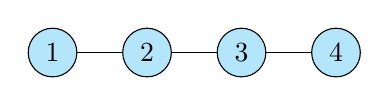
\begin{tikzpicture}[
    vertex/.style={circle, draw, minimum size=0.6cm, fill=cyan!30}
]
    \node[vertex] (1) at (0, 0) {1};
    \node[vertex] (2) at (1.2, 0) {2};
    \node[vertex] (3) at (2.4, 0) {3};
    \node[vertex] (4) at (3.6, 0) {4};
    \draw (1) -- (2) -- (3) -- (4);
\end{tikzpicture}
\end{center}

路径图 $P_4$ 的邻接矩阵为：
\[
A = \begin{pmatrix}
0 & 1 & 0 & 0 \\
1 & 0 & 1 & 0 \\
0 & 1 & 0 & 1 \\
0 & 0 & 1 & 0
\end{pmatrix}
\]

\textbf{性质：}
\begin{itemize}
    \item \textbf{对角线元素都是 0}（简单图没有环）
    \item 矩阵是\textbf{对称矩阵}（邻接关系是对称的）
\end{itemize}
\end{example}

%----------------------------------------
% 图同构
%----------------------------------------

\newpage
\subsection{图同构}

两个图\textbf{相同}（same）当且仅当：
\begin{itemize}
    \item 它们具有\textbf{相同的顶点集合}
    \item 以及\textbf{相同的边集合}
\end{itemize}

然而，两个图可以有\textbf{不同的顶点标签}，但\textbf{结构相同}。这就引出了\textbf{图同构}的概念。

\begin{definition}[图同构]
两个简单图 $G_1$ 和 $G_2$ \textbf{同构}（isomorphic），记作 $G_1 \cong G_2$，如果存在一个\textbf{双射} $\phi: V(G_1) \to V(G_2)$，使得：
\[
uv \in E(G_1) \iff \phi(u)\phi(v) \in E(G_2)
\]
\end{definition}

\textbf{直观理解：} 两个图同构，如果\textbf{只需要重新标记顶点}（relabel vertices）就能把一个图变成另一个图。

\begin{example}[同构图示例]
图 1.2 展示了五个不同的图：
\begin{itemize}
    \item 左边三个图\textbf{互相同构}
    \item 右边两个图\textbf{互相同构}
\end{itemize}

\begin{center}
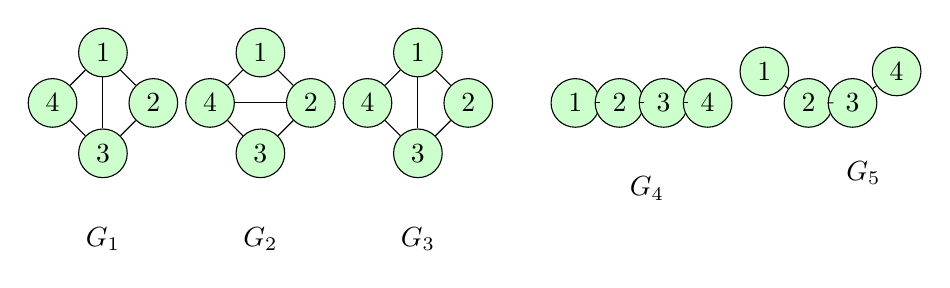
\begin{tikzpicture}[
    vertex/.style={circle, draw, minimum size=0.5cm, fill=green!20},
    scale=0.8
]
    % G1: 正方形
    \begin{scope}[shift={(0,0)}]
        \node[vertex] (1) at (0, 0.8) {1};
        \node[vertex] (2) at (0.8, 0) {2};
        \node[vertex] (3) at (0, -0.8) {3};
        \node[vertex] (4) at (-0.8, 0) {4};
        \draw (1) -- (2) -- (3) -- (4) -- (1);
        \draw (1) -- (3);
        \node[below=0.5cm of 3] {$G_1$};
    \end{scope}

    % G2: 菱形
    \begin{scope}[shift={(2.5,0)}]
        \node[vertex] (1) at (0, 0.8) {1};
        \node[vertex] (2) at (0.8, 0) {2};
        \node[vertex] (3) at (0, -0.8) {3};
        \node[vertex] (4) at (-0.8, 0) {4};
        \draw (1) -- (2);
        \draw (2) -- (3);
        \draw (3) -- (4);
        \draw (4) -- (1);
        \draw (2) -- (4);
        \node[below=0.5cm of 3] {$G_2$};
    \end{scope}

    % G3: K4去掉一条边
    \begin{scope}[shift={(5,0)}]
        \node[vertex] (1) at (0, 0.8) {1};
        \node[vertex] (2) at (0.8, 0) {2};
        \node[vertex] (3) at (0, -0.8) {3};
        \node[vertex] (4) at (-0.8, 0) {4};
        \draw (1) -- (2);
        \draw (1) -- (3);
        \draw (1) -- (4);
        \draw (2) -- (3);
        \draw (3) -- (4);
        \node[below=0.5cm of 3] {$G_3$};
    \end{scope}

    % G4: 路径
    \begin{scope}[shift={(7.5,0)}]
        \node[vertex] (1) at (0, 0) {1};
        \node[vertex] (2) at (0.7, 0) {2};
        \node[vertex] (3) at (1.4, 0) {3};
        \node[vertex] (4) at (2.1, 0) {4};
        \draw (1) -- (2) -- (3) -- (4);
        \node[below=0.5cm of 2, xshift=0.35cm] {$G_4$};
    \end{scope}

    % G5: 弯曲路径
    \begin{scope}[shift={(10.5,0)}]
        \node[vertex] (1) at (0, 0.5) {1};
        \node[vertex] (2) at (0.7, 0) {2};
        \node[vertex] (3) at (1.4, 0) {3};
        \node[vertex] (4) at (2.1, 0.5) {4};
        \draw (1) -- (2) -- (3) -- (4);
        \node[below=0.3cm of 2, xshift=0.7cm] {$G_5$};
    \end{scope}
\end{tikzpicture}
\end{center}

\textbf{注意：} 虽然 $G_1, G_2, G_3$ 的画法不同，但它们实际上是\textbf{同一个图结构}（$K_4$ 减去一条边）。
\end{example}

\begin{example}[验证同构]
验证 $G_1 \cong G_2$：考虑映射 $\phi: V(G_1) \to V(G_2)$：
\[
\phi(1) = 2, \quad \phi(2) = 3, \quad \phi(3) = 4, \quad \phi(4) = 1
\]

验证：对于所有 $u, v$，$uv \in E(G_1)$ 当且仅当 $\phi(u)\phi(v) \in E(G_2)$。

例如：
\begin{itemize}
    \item $12 \in E(G_1)$，且 $\phi(1)\phi(2) = 23 \in E(G_2)$ \checkmark
    \item $14 \in E(G_1)$，且 $\phi(1)\phi(4) = 21 \in E(G_2)$ \checkmark
    \item $13 \in E(G_1)$，但 $\phi(1)\phi(3) = 24 \in E(G_2)$（对角线）\checkmark
\end{itemize}

因此 $G_1 \cong G_2$。
\end{example}

\textbf{判断同构的技巧：}
\begin{itemize}
    \item 检查顶点数和边数是否相同
    \item 检查度数序列是否相同
    \item 尝试找到保持邻接关系的顶点对应
\end{itemize}

\subsubsection{图同构的必要条件}

两个图 $G_1$ 和 $G_2$ 同构的\textbf{必要条件}：
\begin{enumerate}
    \item 两个图必须\textbf{具有相同数量的顶点}：$|V(G_1)| = |V(G_2)|$
    \item 两个图必须\textbf{具有相同数量的边}：$|E(G_1)| = |E(G_2)|$
    \item 两个图中\textbf{每种度数的顶点数量相同}
    \item 两个图必须具有\textbf{相同的度序列}（degree sequence）
    \item 两个图必须具有\textbf{相同的循环向量}（cycle vector）$(c_1, \dots, c_n)$，其中 $c_i$ 表示长度为 $i$ 的环的数量
\end{enumerate}

\textbf{注意：} 判断两个图是否同构\textbf{并不简单}，因为我们必须找到一个合适的双射，或证明不存在这样的双射。

\subsubsection{同构不变量}

有些图的性质在\textbf{同构变换下保持不变}，这些性质称为\textbf{同构不变量}（isomorphism invariants）。

\textbf{常见的同构不变量：}
\begin{itemize}
    \item 顶点数、边数
    \item 度序列
    \item 环的数量和长度
    \item 连通性
    \item 图的直径、半径
\end{itemize}

\textbf{传递性：} 图同构是一种\textbf{等价关系}，满足传递性。例如，如果 $G_1 \cong G_2$ 且 $G_2 \cong G_3$，则 $G_1 \cong G_3$。

%----------------------------------------
% 子图
%----------------------------------------

\newpage
\subsection{子图}

有时候我们希望讨论一个图的\textbf{较小部分}，为此引入\textbf{子图}的概念。

\begin{definition}[子图]
设 $G$ 是一个图。如果 $V(H) \subseteq V(G)$ 且 $E(H) \subseteq E(G)$，则图 $H$ 称为\textbf{图 $G$ 的子图}。

\textbf{注意：} 由于 $H$ 必须本身也是一个图，因此 $E(H)$ 中的每一条边必须连接 $V(H)$ 中的顶点。
\end{definition}

\textbf{构造子图的两种方法：}

\textbf{步骤 1：} 从顶点集合 $V$ 中删除一些顶点，同时删除所有与这些顶点相关联的边。

\textbf{步骤 2：} 从剩余的边集合中删除任意一些边。

\begin{example}[子图示例]
\begin{center}
\begin{tikzpicture}[
    vertex/.style={circle, draw, minimum size=0.6cm},
    main/.style={vertex, fill=blue!20},
    sub/.style={vertex, fill=orange!30}
]
    % 原图 G
    \begin{scope}[shift={(0,0)}]
        \node[main] (1) at (0, 1) {1};
        \node[main] (2) at (1.5, 1) {2};
        \node[main] (3) at (0, 0) {3};
        \node[main] (4) at (1.5, 0) {4};
        \node[main] (5) at (0.75, -1) {5};
        \draw (1) -- (2) -- (4) -- (3) -- (1);
        \draw (2) -- (3);
        \draw (3) -- (5) -- (4);
        \node[below=0.3cm of 5] {原图 $G$};
    \end{scope}

    % 子图 1
    \begin{scope}[shift={(4,0)}]
        \node[sub] (1) at (0, 1) {1};
        \node[sub] (2) at (1.5, 1) {2};
        \node[sub] (3) at (0, 0) {3};
        \node[sub] (4) at (1.5, 0) {4};
        \draw (1) -- (2) -- (4) -- (3) -- (1);
        \draw (2) -- (3);
        \node[below=0.5cm of 3, xshift=0.75cm] {子图（删除顶点 5）};
    \end{scope}

    % 子图 2
    \begin{scope}[shift={(8,0)}]
        \node[sub] (1) at (0, 1) {1};
        \node[sub] (2) at (1.5, 1) {2};
        \node[sub] (3) at (0, 0) {3};
        \node[sub] (4) at (1.5, 0) {4};
        \draw (1) -- (2);
        \draw (3) -- (4);
        \node[below=0.5cm of 3, xshift=0.75cm] {子图（再删除边）};
    \end{scope}
\end{tikzpicture}
\end{center}
\end{example}

\begin{definition}[诱导子图]
设 $G$ 是一个图，且 $X \subseteq V(G)$。图 $G$ 在顶点集合 $X$ 上的\textbf{诱导子图}记为 $G[X]$，其中：
\begin{itemize}
    \item $V(H) = X$
    \item $E(H)$ 包含\textbf{所有在 $G$ 中连接 $X$ 中顶点的边}
\end{itemize}
\end{definition}

\begin{example}[诱导子图 vs 普通子图]
\begin{center}
\begin{tikzpicture}[
    vertex/.style={circle, draw, minimum size=0.5cm},
    main/.style={vertex, fill=blue!20},
    induced/.style={vertex, fill=red!30},
    normal/.style={vertex, fill=yellow!30}
]
    % 原图 G
    \begin{scope}[shift={(0,0)}]
        \node[main] (1) at (0, 0.8) {1};
        \node[main] (2) at (0.8, 0) {2};
        \node[main] (3) at (0, -0.8) {3};
        \node[main] (4) at (-0.8, 0) {4};
        \draw (1) -- (2) -- (3) -- (4) -- (1);
        \draw (1) -- (3);
        \draw (2) -- (4);
        \node[below=0.6cm of 3] {原图 $G$};
    \end{scope}

    % 诱导子图
    \begin{scope}[shift={(3,0)}]
        \node[induced] (1) at (0, 0.8) {1};
        \node[induced] (2) at (0.8, 0) {2};
        \node[induced] (3) at (0, -0.8) {3};
        \node[induced] (4) at (-0.8, 0) {4};
        \draw (1) -- (2) -- (3) -- (4) -- (1);
        \draw (1) -- (3);
        \draw (2) -- (4);
        \node[below=0.6cm of 3] {诱导子图 $G[\{1,2,3,4\}]$};
    \end{scope}

    % 普通子图（非诱导）
    \begin{scope}[shift={(6,0)}]
        \node[normal] (1) at (0, 0.8) {1};
        \node[normal] (2) at (0.8, 0) {2};
        \node[normal] (3) at (0, -0.8) {3};
        \node[normal] (4) at (-0.8, 0) {4};
        \draw (1) -- (2) -- (3) -- (4) -- (1);
        \draw (2) -- (4);
        % 缺少边 1-3
        \node[below=0.6cm of 3] {普通子图（缺少边 1-3）};
    \end{scope}
\end{tikzpicture}
\end{center}

\textbf{关键区别：}
\begin{itemize}
    \item \textbf{诱导子图}：保留 $X$ 中所有顶点之间的边
    \item \textbf{普通子图}：可以删除一些边
\end{itemize}
\end{example}

\textbf{注意：} 任何图都是它自己的子图，同时也是它自己的诱导子图。

\subsubsection{子图的并集与交集}

给定图 $G$ 及其两个子图 $G_1$ 和 $G_2$：

\textbf{并集子图} $G_1 \cup G_2$：
\[
V(G_1 \cup G_2) = V(G_1) \cup V(G_2), \quad E(G_1 \cup G_2) = E(G_1) \cup E(G_2)
\]

\textbf{交集子图} $G_1 \cap G_2$：
\[
V(G_1 \cap G_2) = V(G_1) \cap V(G_2), \quad E(G_1 \cap G_2) = E(G_1) \cap E(G_2)
\]

%----------------------------------------
% 邻域与度
%----------------------------------------

\newpage
\subsection{邻域与度}

如果我们从\textbf{某个特定顶点的角度}来观察一个图，那么两个重要的对象是：
\begin{itemize}
    \item \textbf{它的邻居是谁}
    \item \textbf{它有多少个邻居}
\end{itemize}

\begin{definition}[邻域]
顶点 $v$ 的\textbf{邻域}（neighborhood）$N(v)$ 是所有与 $v$ 邻接的顶点的集合：
\[
N(v) = \{u \in V(G) : uv \in E(G)\}
\]
\end{definition}

\begin{definition}[度数]
顶点 $v$ 的\textbf{度数}（degree）$\deg(v)$ 是其邻域中顶点的数量：
\[
\deg(v) = |N(v)|
\]

\textbf{特殊情况：}
\begin{itemize}
    \item 若 $\deg(v) = 0$，则 $v$ 是\textbf{孤立顶点}（isolated vertex）
    \item 若 $\deg(v) = 1$，则 $v$ 是\textbf{悬挂顶点}（pendant vertex / leaf）
    \item 环对度数的贡献为 2
\end{itemize}
\end{definition}

\begin{example}[邻域与度数示例]
\begin{center}
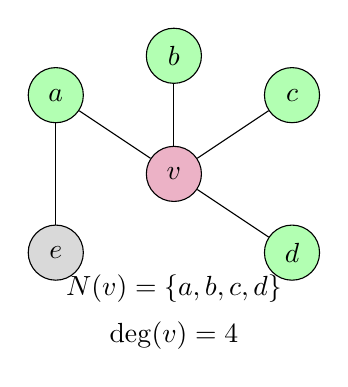
\begin{tikzpicture}[
    vertex/.style={circle, draw, minimum size=0.7cm},
    main/.style={vertex, fill=purple!30},
    neighbor/.style={vertex, fill=green!30}
]
    \node[main] (v) at (0, 0) {$v$};
    \node[neighbor] (a) at (-1.5, 1) {$a$};
    \node[neighbor] (b) at (0, 1.5) {$b$};
    \node[neighbor] (c) at (1.5, 1) {$c$};
    \node[neighbor] (d) at (1.5, -1) {$d$};
    \node[vertex, fill=gray!30] (e) at (-1.5, -1) {$e$};

    \draw (v) -- (a);
    \draw (v) -- (b);
    \draw (v) -- (c);
    \draw (v) -- (d);
    \draw (a) -- (e);

    \node[below=0.8cm of v] {$N(v) = \{a, b, c, d\}$};
    \node[below=1.4cm of v] {$\deg(v) = 4$};
\end{tikzpicture}
\end{center}

\textbf{说明：} 紫色顶点 $v$ 的邻域是绿色顶点 $\{a, b, c, d\}$，度数为 4。灰色顶点 $e$ 不是 $v$ 的邻居。
\end{example}

%----------------------------------------
% 度矩阵与拉普拉斯矩阵
%----------------------------------------

\newpage
\subsection{图矩阵}

我们已经介绍了\textbf{关联矩阵}、\textbf{邻接矩阵}和\textbf{距离矩阵}。本节介绍更多与图相关的矩阵。

\textbf{矩阵分析与图论联系紧密}，在证明许多结论时，使用矩阵往往更加方便。

\begin{definition}[度矩阵]
给定图 $G = (V, E)$，且 $|V| = n$，图 $G$ 的\textbf{度矩阵} $D$ 是一个 $n \times n$ 的\textbf{对角矩阵}：
\[
D_{ij} = \begin{cases}
\deg(v_i) & i = j \\
0 & \text{otherwise}
\end{cases}
\]

\textbf{注意：}
\begin{itemize}
    \item 在\textbf{无向图}中：每个自环对度贡献为 2
    \item 在\textbf{有向图}中：度可能指入度或出度
\end{itemize}
\end{definition}

\begin{definition}[拉普拉斯矩阵]
设 $V(G) = \{1, \dots, n\}$，$E(G) = \{e_1, \dots, e_m\}$。记 $A(G)$ 为图 $G$ 的邻接矩阵：
\[
A_{ij} = \begin{cases}
1 & i \sim j \\
0 & \text{otherwise}
\end{cases}
\]

其中 $D(G) = \text{diag}(d_1, \dots, d_n)$ 表示顶点度的对角矩阵。

图 $G$ 的\textbf{拉普拉斯矩阵}定义为：
\[
L(G) = D(G) - A(G)
\]
\end{definition}

\begin{example}[拉普拉斯矩阵示例]
对于图 $G$：
\begin{center}
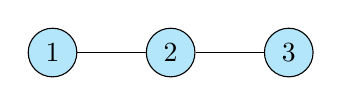
\begin{tikzpicture}[
    vertex/.style={circle, draw, minimum size=0.6cm, fill=cyan!30}
]
    \node[vertex] (1) at (0, 0) {1};
    \node[vertex] (2) at (1.5, 0) {2};
    \node[vertex] (3) at (3, 0) {3};
    \draw (1) -- (2) -- (3);
\end{tikzpicture}
\end{center}

度矩阵：$D = \begin{pmatrix} 1 & 0 & 0 \\ 0 & 2 & 0 \\ 0 & 0 & 1 \end{pmatrix}$，邻接矩阵：$A = \begin{pmatrix} 0 & 1 & 0 \\ 1 & 0 & 1 \\ 0 & 1 & 0 \end{pmatrix}$

拉普拉斯矩阵：$L = D - A = \begin{pmatrix} 1 & -1 & 0 \\ -1 & 2 & -1 \\ 0 & -1 & 1 \end{pmatrix}$
\end{example}

%----------------------------------------
% 有向图与网络
%----------------------------------------

\newpage
\subsection{有向图与网络}

在某些情况下，\textbf{关系的方向}也很重要，这就引出了\textbf{有向图}的概念。

\begin{definition}[有向图]
有向图 $D$ 是一种图，其中每条边 $e$ 都被赋予\textbf{方向}：从一个端点 $u$ 指向另一个端点 $v$。

此时称该边为\textbf{弧}（arc），从 $u$ 指向 $v$。
\begin{itemize}
    \item $u$ 称为\textbf{尾}（tail）
    \item $v$ 称为\textbf{头}（head）
\end{itemize}

若给定有向图 $D$，则 $A(D)$ 表示弧的集合。每个弧对应一个\textbf{有序顶点对}。
\end{definition}

\begin{definition}[出度与入度]
设有向图 $D$，且 $v \in V(D)$。
\begin{itemize}
    \item \textbf{出度} $d^+(v)$：尾为 $v$ 的弧数量
    \item \textbf{入度} $d^-(v)$：头为 $v$ 的弧数量
\end{itemize}
\end{definition}

\begin{lemma}[有向图的握手引理]
对于任意有向图 $D$：
\[
\sum_{v \in V(D)} d^+(v) = \sum_{v \in V(D)} d^-(v) = |A(D)|
\]
\end{lemma}

\begin{definition}[网络]
一个\textbf{网络}是图或有向图 $G$ 加上一个函数 $w: E(G) \to \mathbb{R}$，给每条边（或弧）赋予一个\textbf{权重}。
\end{definition}

\begin{center}
\begin{tikzpicture}[
    vertex/.style={circle, draw, minimum size=0.6cm, fill=orange!20},
    ->.style={thick, ->, >=stealth}
]
    \node[vertex] (A) at (0, 0) {$A$};
    \node[vertex] (B) at (2, 1) {$B$};
    \node[vertex] (C) at (2, -1) {$C$};
    \node[vertex] (D) at (4, 0) {$D$};

    \draw[->] (A) -- node[midway, above] {$3$} (B);
    \draw[->] (A) -- node[midway, below] {$2$} (C);
    \draw[->] (B) -- node[midway, above] {$4$} (D);
    \draw[->] (C) -- node[midway, below] {$1$} (D);
\end{tikzpicture}
\end{center}

\textbf{说明：} 有向网络示例，箭头表示方向
数字表示权重。

有向图的\textbf{邻接矩阵}是 $|V(D)| \times |V(D)|$ 矩阵。如果 $uv \in A(D)$
则矩阵第 $u$ 行第 $v$ 列为 1。

\textbf{注意：} 与无向图不同，有向图的邻接矩阵\textbf{通常不是对称的}。

对于网络，矩阵中的元素可以直接表示权重。但需要区分：
\begin{itemize}
    \item 权重为 0 的边
    \item 不存在的边（通常用 $\infty$ 表示）
\end{itemize}

%----------------------------------------
% 第二章：路径、环和树
%----------------------------------------

\newpage
\section{路径、环和树}

我们现在不再只关注一个顶点的邻域
而是研究\textbf{通过一系列边可以到达的顶点}。这个概念通过\textbf{walk}及其各种特殊形式来描述。

\begin{definition}[Walk,Trail
Path
Cycle]
在图中：
\begin{itemize}
    \item \textbf{Walk（游走）}：顶点和边交替出现的序列，每条边前后都是它的端点。Walk 的\textbf{长度}等于序列中的边数。
    \item \textbf{u-v walk}：从顶点 $u$ 开始，在顶点 $v$ 结束的 walk
    \item \textbf{Closed walk（闭游走）}：起点 = 终点的 walk
    \item \textbf{Trail（迹）}：所有边都不同的 walk
    \item \textbf{Path（路径）}：所有顶点都不同的 walk
    \item \textbf{Tour（巡游）}：闭迹
    \item \textbf{Cycle（环）}：一个 tour，并且至少包含一条边
除了首尾顶点外，其余所有顶点都不同
\end{itemize}

\textbf{有向版本：} 在有向图中
每条弧都必须从尾到头。
\end{definition}

\textbf{另一种定义方式：}
\begin{itemize}
    \item 长度为 $k$ 的 \textbf{path} 可以定义为 $G$ 的一个子图
该子图与 $P_{k+1}$ 同构
    \item 长度为 $k$ 的 \textbf{cycle} 可以定义为 $G$ 的一个子图
该子图与 $C_k$ 同构
\end{itemize}

%----------------------------------------
% 连通性
%----------------------------------------

\newpage
\subsection{连通性}

直观地说
在图 $G$ 中存在一条 \textbf{u-v path}
意味着可以通过沿着图 $G$ 的边行走
从顶点 $u$ 到达顶点 $v$。

\begin{definition}[连通图]
如果对于每一对顶点 $u, v \in V(G)$
在 $G$ 中都存在一条 \textbf{u-v walk}
则称图 $G$ 是\textbf{连通的}（connected）。
\end{definition}

\begin{lemma}[Path 与 Walk 的等价性]
设 $G$ 为一个图，且 $u, v \in V(G)$。那么
在 $G$ 中\textbf{存在一条 u-v path} 当且仅当\textbf{存在一条 u-v walk}。
\end{lemma}

\textbf{证明思路：} 从左到右是显然的（每条 path 也是 walk）。对于从右到左
设 $W$ 是长度最小的 u-v walk。如果 $W$ 不是 path
则某个顶点出现多于一次
可以删除重复部分得到更短的 walk
矛盾。

\begin{corollary}[连通性的等价定义]
图 $G$ 是\textbf{连通的}
当且仅当对于每一对顶点 $u, v \in V(G)$
在 $G$ 中都存在一条 \textbf{u-v path}。
\end{corollary}

\begin{definition}[连通分量]
图 $G$ 的一个\textbf{连通分量}（connected component）是 $G$ 的一个\textbf{极大连通子图}
也就是说
它是一个连通子图
并且不是任何其他更大的连通子图的子图。
\end{definition}

\textbf{注意：} 一个\textbf{连通图}只有一个连通分量
这个连通分量就是图本身。

\begin{example}[连通与不连通图]
\begin{center}
\begin{tikzpicture}[
    vertex/.style={circle, draw, minimum size=0.5cm},
    connected/.style={vertex, fill=green!30},
    disconnected/.style={vertex, fill=red!20}
]
    % G1: 连通图
    \begin{scope}[shift={(0,0)}]
        \node[connected] (1) at (0, 0.6) {1};
        \node[connected] (2) at (0.8, 0) {2};
        \node[connected] (3) at (0, -0.6) {3};
        \node[connected] (4) at (-0.8, 0) {4};
        \draw (1) -- (2) -- (3) -- (4) -- (1);
        \draw (1) -- (3);
        \draw (2) -- (4);
        \node[below=0.5cm of 3] {连通图 $G_1$};
    \end{scope}

    % G2: 不连通图（两个连通分量）
    \begin{scope}[shift={(3,0)}]
        \node[disconnected] (1) at (0, 0.4) {1};
        \node[disconnected] (2) at (0.6, 0) {2};
        \node[disconnected] (3) at (0, -0.4) {3};
        \draw (1) -- (2) -- (3) -- (1);

        \node[disconnected] (4) at (1.5, 0.4) {4};
        \node[disconnected] (5) at (2.1, 0) {5};
        \node[disconnected] (6) at (1.5, -0.4) {6};
        \draw (4) -- (5) -- (6) -- (4);

        \node[below=0.5cm of 3, xshift=0.3cm] {不连通图 $G_2$};
        \node[below=1cm of 3, xshift=0.3cm, font=\small] {（两个连通分量）};
    \end{scope}
\end{tikzpicture}
\end{center}
\end{example}

\begin{lemma}[连通子图的并集]
设 $G$ 是一个图
并考虑 $G$ 的两个连通子图 $G_1$ 和 $G_2$
满足 $V(G_1) \cap V(G_2) \ne \varnothing$。则 $G_1 \cup G_2$ 是\textbf{连通的}。
\end{lemma}

\begin{lemma}[连通分量划分顶点和边]
设图 $G$ 的连通分量为 $G_1, \dots, G_m$。则：
\begin{itemize}
    \item $\{V(G_1), \dots, V(G_m)\}$ 构成 $V(G)$ 的一个\textbf{划分}
    \item $\{E(G_1), \dots, E(G_m)\}$ 构成 $E(G)$ 的一个\textbf{划分}
\end{itemize}

\textbf{换句话说：}
\begin{itemize}
    \item 每个顶点\textbf{属于且只属于一个连通分量}
    \item 每条边\textbf{属于且只属于一个连通分量}
\end{itemize}
\end{lemma}

\textbf{有向图的更强连通概念：} 可以要求任意两个顶点之间存在\textbf{有向路径}。

%----------------------------------------
% 第二章：图的遍历
%----------------------------------------

\newpage
\section{图的遍历}

\subsection{深度优先搜索 (DFS)}

\begin{center}
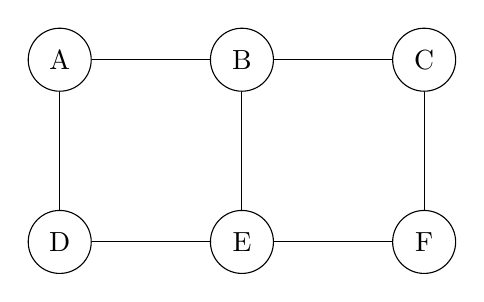
\begin{tikzpicture}[
    node distance=1.5cm,
    vertex/.style={circle, draw, minimum size=0.8cm}
]
    \node[vertex] (A) {A};
    \node[vertex, right=of A] (B) {B};
    \node[vertex, right=of B] (C) {C};
    \node[vertex, below=of A] (D) {D};
    \node[vertex, below=of B] (E) {E};
    \node[vertex, below=of C] (F) {F};

    \draw (A) -- (B);
    \draw (B) -- (C);
    \draw (A) -- (D);
    \draw (B) -- (E);
    \draw (C) -- (F);
    \draw (D) -- (E);
    \draw (E) -- (F);
\end{tikzpicture}
\end{center}

DFS 从起点出发，沿着一条路径尽可能深入，直到无法继续，然后回溯。

\textbf{时间复杂度：} $O(|V| + |E|)$

\subsection{广度优先搜索 (BFS)}

BFS 按层级遍历图，先访问距离起点最近的顶点。

\textbf{时间复杂度：} $O(|V| + |E|)$

%----------------------------------------
% 第三章：最短路径算法
%----------------------------------------

\newpage
\section{最短路径算法}

\subsection{Dijkstra 算法}

适用于\textbf{非负权图}的单源最短路径。

\begin{center}
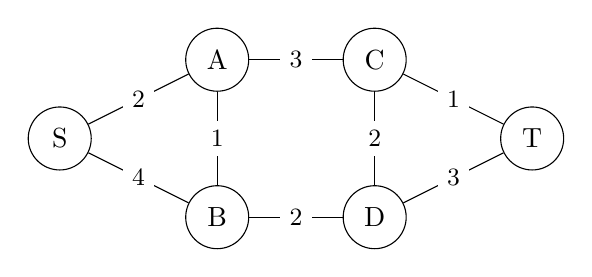
\begin{tikzpicture}[
    vertex/.style={circle, draw, minimum size=0.8cm},
    weight/.style={midway, fill=white, font=\small}
]
    \node[vertex] (S) at (0, 0) {S};
    \node[vertex] (A) at (2, 1) {A};
    \node[vertex] (B) at (2, -1) {B};
    \node[vertex] (C) at (4, 1) {C};
    \node[vertex] (D) at (4, -1) {D};
    \node[vertex] (T) at (6, 0) {T};

    \draw (S) -- node[weight] {2} (A);
    \draw (S) -- node[weight] {4} (B);
    \draw (A) -- node[weight] {3} (C);
    \draw (A) -- node[weight] {1} (B);
    \draw (B) -- node[weight] {2} (D);
    \draw (C) -- node[weight] {1} (T);
    \draw (D) -- node[weight] {3} (T);
    \draw (C) -- node[weight] {2} (D);
\end{tikzpicture}
\end{center}

\textbf{时间复杂度：}
\begin{itemize}
    \item 朴素实现：$O(|V|^2)$
    \item 优先队列：$O((|V| + |E|) \log |V|)$
\end{itemize}

%----------------------------------------
% 第四章：最小生成树
%----------------------------------------

\newpage
\section{最小生成树}

\subsection{Prim 算法}

从任意顶点开始，每次选择连接已选顶点和未选顶点的最小权边。

\subsection{Kruskal 算法}

按边权排序，依次选择不形成环的最小权边。

\begin{center}
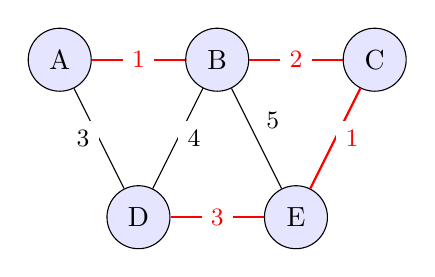
\begin{tikzpicture}[
    vertex/.style={circle, draw, minimum size=0.8cm, fill=blue!10},
    mst/.style={red, thick},
    weight/.style={midway, fill=white, font=\small}
]
    \node[vertex] (A) at (0, 2) {A};
    \node[vertex] (B) at (2, 2) {B};
    \node[vertex] (C) at (4, 2) {C};
    \node[vertex] (D) at (1, 0) {D};
    \node[vertex] (E) at (3, 0) {E};

    \draw[mst] (A) -- node[weight] {1} (B);
    \draw (A) -- node[weight, left] {3} (D);
    \draw[mst] (B) -- node[weight] {2} (C);
    \draw (B) -- node[weight, right] {4} (D);
    \draw (B) -- node[weight, above right] {5} (E);
    \draw[mst] (C) -- node[weight, right] {1} (E);
    \draw[mst] (D) -- node[weight] {3} (E);
\end{tikzpicture}
\end{center}

\textbf{红色边}为最小生成树的边，总权重 $= 1 + 2 + 1 + 3 = 7$。

\textbf{时间复杂度：} $O(|E| \log |E|)$（使用并查集）

%========================================
% 继续添加更多章节...
%========================================

\end{document}
